\documentclass[a4paper, 10pt, twocolumn, twoside]{article}

\usepackage{ISARC}

\usepackage{lscape}
\usepackage{hologo}
\usepackage{multirow}

\begin{document}

 % Do not change the following line
\linespread{0.5}

\title{BIM-FM interoperability: integrating existing FM platform with visualization of IFC models}

\author{Andressa Oliveira$^{1}$, José Granja$^1$, Pedro Machado$^2$, Ali Motamedi$^3$, and Miguel Azenha$^1$}

\affiliation{
$^1$University of Minho, ISISE, ARISE, Department of Civil Engineering, Portugal\\
$^2$Matosinhos City Council, Portugal\\
$^2$Université du Québec à Montreal, École de Technologie Supérieure, Canada
}

\email{
\href{mailto:soliveira.andressa@gmail.com}{Email Andressa Oliveira}, 
\href{mailto:granja@civil.uminho.pt}{Email José Granja},
\href{mailto:pedro.machado@cm-matosinhos.pt}{Email Pedro Machado},
\href{mailto:ali.motamedi@etsmtl.ca}{Email Ali Motamedi},
\href{mailto:miguel.azenha@gmail.com}{Email Miguel Azenha}
}


% Do not change the following three lines
\maketitle 
\thispagestyle{fancy} 
\pagestyle{fancy}

\begin{abstract}
The adoption of Building Information Modelling (BIM) in building operations is limited, mostly due to insufficient BIM capabilities in Facility Management (FM) platforms. This article shows the developments derived from a collaboration with the Matosinhos City Hall in Portugal. The collaboration included the development of a customized web platform to integrate the existing management software (Infraspeak), already in use by the town hall, with 3D visualization capabilities, and developing information requirements to guide the preparation of information models to be visualized on the platform. The platform enables the visualization of 3D models developed according to the IFC (Industry Foundation Classes) schema using the IFCjs library to manipulate, investigate and visualize IFC files. In addition, the web platform enables direct access to and manipulation of operational data through the 3D model. The framework presented in this paper shows how the IFC model elements are linked to the Infraspeak database through its API. This solution addresses current operational limitations and promotes broader BIM adoption in the FM sector.
\end{abstract}

\begin{keywords}
Facility Management (FM); Building Information Modelling (BIM); Interoperability; Integration; Web Platform
\end{keywords}

% AS SESSÕES DO ARTIGO COMEÇAM AQUI

\section{Introduction}
\label{sec:Introduction}

Facility Management (FM) ensures the functionality, comfort, and safety of facilities in the built environment \cite{IFMA2023} and is rapidly growing within the construction sector \cite{Pinti2022}. As facility managers increasingly adopt the BIM methodology to enhance operations \cite{Marocco2021}, the complexity of assets in public and large buildings presents unique challenges \cite{Pinti2022}. Despite the various advantages found in the literature, there is still resistance to adopting BIM for asset operation \cite{Durdyev2022}, and managers are faced with buildings already in the operational phase but not yet managed with the support of the BIM methodology.

For broader adoption of BIM in FM, it is essential to enhance knowledge of its information management processes in line with ISO 19650 series guidelines and to adapt management systems for emerging technologies \cite{Durdyev2022}. The use of computerized management platforms like Intelligent Maintenance Management Platform (IMMP) for operating built assets is already widespread \cite{Marocco2021, Siccardi2023}. However, it is necessary to employ platforms capable of integrating various data sources, particularly information models \cite{Al-Kasasbeh2021}. These models, which include three-dimensional representations of assets, should be prepared to integrate with management platforms used by operational managers.

From this context, a collaboration between Matosinhos City Hall (CMMatosinhos) in Portugal and the University of Minho (UMinho) aimed to enhance municipal asset management by integrating BIM methodology into the Infraspeak management platform already used by CMMatosinhos. While Infraspeak allows users to access functionalities via a web interface and API, it lacks the capability to visualize managed buildings and assets. The project aimed to develop a web platform that integrates the IMMP database with three-dimensional visualization, enabling users to consult, edit, and add information about the assets.  This collaboration will enable CMMatosinhos to integrate geometric information into decision-making. For example, visually mapping equipment needing maintenance will help establish more efficient action routes. The platform integrates two key data sources: the IMMP database with essential asset operation information and the information model containing geometrical data for buildings and assets.

\section{Methodology and functional requirements for the platform}
\label{sec:methodology}

The partnership required the development of a platform capable of integrating the IMMP used by CMMatosinhos with the ability to visualize and manipulate three-dimensional models of buildings under its management. It also encompasses the definition of information requirements for models to be used within this platform. Meetings with the town hall allowed a detailed understanding of its objectives with the platform, which were necessary to establish its foreseen functionalities. Initially, the platform should provide a building selection interface. The platform should support comprehensive 3D visualization options, including viewing the entire building, individual floors, or specific elements with open requests. Additionally, users should be able to interact with the 3D model by selecting assets directly from the 3D representation. The platform should display the building's identification details and the number of open requests linked to it. For asset-specific information, the platform should allow users to identify assets through selection and display the total number of open requests associated with a particular asset. Furthermore, it should include a feature to redirect manager users to the asset's IMMP dedicated page for more in-depth information. Lastly, the platform should allow users to submit requests associated with specific assets.

From the functionalities, it was established that the web platform would contain two pages: the building selection page and the interaction page. Regarding the users, it would include two different user profiles (manager and common user). Both user profiles would allow users to visualize the building, interact with its 3D representation, see identification information about the building and its assets, and submit requests related to assets (equipment or spaces). In addition, the manager user profile would be able to visualize information regarding the open requests related to the building, spaces, or assets and be redirected to specific pages of the IMMP. The development of the web platform can be divided into two layers: frontend and backend. HTML, CSS and JavaScript were used for the frontend. Among the platform's functionalities, those related to dealing with the IFC model were developed with the support of the IFCjs open-source library. This library allows the creation of customised and interactive viewers, including viewing the entire building or subsets of it and selecting specific elements within the model. In addition, the library allows you to access element properties and extract information from them. The backend was developed in Python using the Flask web framework. The prototype building model was developed on the Autodesk Revit 2023 platform and followed previously defined information requirements. This model was then exported following the IFC scheme (IFC4 ADD2 TC1) \cite{BuildingSMARTa}.

\section{Implementation}
\label{sec:implementation}

To develop this work, the 'IMMP database' must be integrated into a web platform presenting the IFC model visualization. The integration is only possible if elements are uniquely identified and associated between the IMMP database and the IFC models (hosted in the 'Models database'). Considering the functionalities to be implemented \ref{sec:methodology}, three types of elements are essential to the platform's objectives: \emph{locations}, \emph{equipment} and \emph{requests}. \emph{Locations} represent spatial assets or spaces that comprise the buildings and are essential to the equipment's localization. \emph{Equipment} is any physical asset from the CMMatosinhos' inventory (vehicles, chairs, ladders, etc.). Finally, \emph{requests} represent the solicitation for an operation action to be carried out and are always associated with the other types of elements (\emph{equipment} or \emph{location}). Figure \ref{fig_fluxo} shows the flow of information between the platform layers (frontend and backend) and how the manager user type interacts with the platform.

\begin{figure}[!htb]
    \centering
    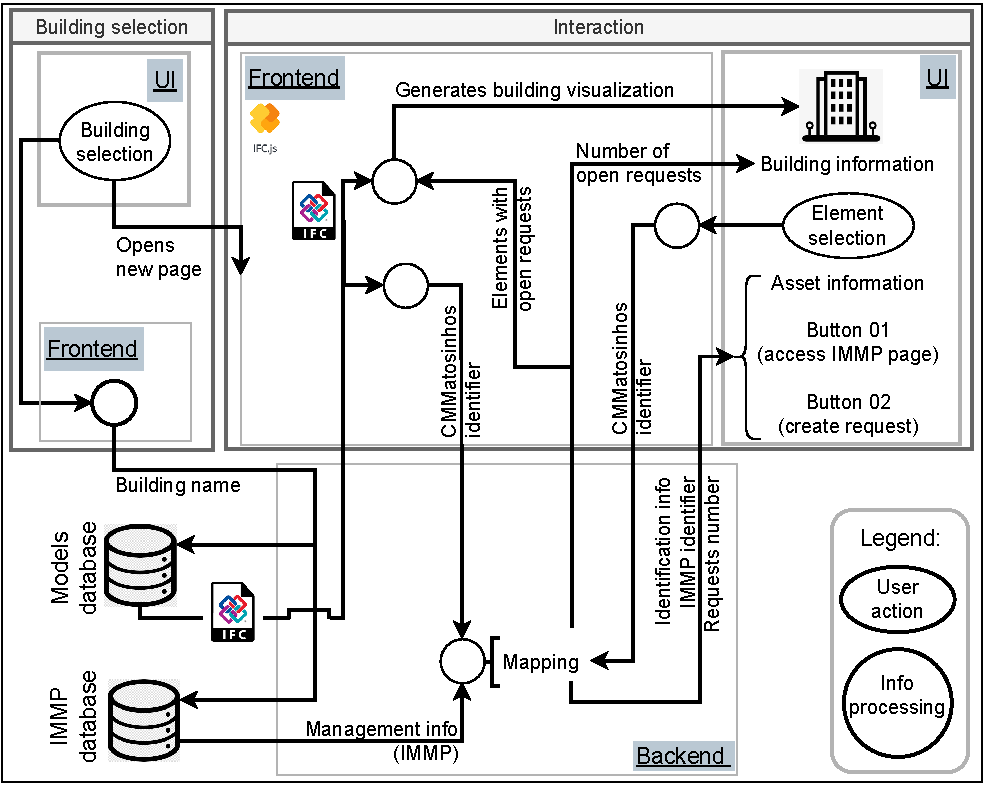
\includegraphics[width=0.48\textwidth]{Images/fluxo.pdf}
    \caption{Information flow on the web platform}
    \label{fig_fluxo}
\end{figure}

\subsection{Unique identifiers}
\label{subsec:identifiers}

To establish the connections between IMMP database and IFC model, it is essential to comprehend how CMMatosinhos identifies them in its inventory (CMMatosinhos identifiers) and how they are represented within the IMMP database (IMMP identifiers). The 'CMMatosinhos identifiers' will be organized as properties to be associated with the model elements (section \ref{subsec:loin}), while the 'IMMP identifiers' will allow the mapping process between the IMMP database and the IFC model.

\paragraph{CMMatosinhos identifier}:

'CMMatosinhos identifiers' relate to the code used by CMMatosinhos to identify its assets within its inventory. Currently, these codes are part of the information associated with the assets within the IMMP database. Therefore, the 'CMMatosinhos identifiers' analysis was conducted using the IMMP database, focusing on attributes that provide information relevant to identifying assets from the CMMatosinhos perspective. Among the three elements (\emph{equipment}, \emph{location}, and \emph{requests}), \emph{requests} do not have a CMMatosinhos identifier as they do not represent physical assets, being not part of CMMatosinhos' inventory. 

As for \emph{locations}, the value of the 'full\_code' attribute represents the codification used by CMMatosinhos to identify spaces hierarchically, containing a unique code for each location. For \emph{equipment}, the value of the 'nfc\_code' attribute was selected as a potential unique identifier. However, not all equipment contains associated NFC codes, which implies that it could not be used as the identification key for this type of asset. In a second analysis, the 'code' attribute was selected for this purpose. Within the CMMatosinhos inventory, the value of this attribute is filled in using a coding specific to the type of equipment (chair, vehicle, etc.) and might not be unique for some specific types of equipment. However, if there is more than one \emph{equipment} element with the same code, those \emph{equipment} would not be in the same space. Therefore, the combination of the attributes 'code' of the equipment and 'full\_code' of the location where it is placed within the model was defined as the 'CMMatosinhos identifier' for the equipment group.

\paragraph{IMMP identifier}:

The IMMP database contains two categories of entries for \emph{locations}: LOCATION and ELEMENT. Within the LOCATION category, they are organized hierarchically and identified by a unique attribute called 'local\_id'. On the other hand, the ELEMENT category includes two types of assets: EQUIPMENT and LOCAL. In this context, the \emph{locations} classified as ELEMENT are specifically of the type LOCAL, representing the lowest level of the spatial hierarchy found in the LOCATION category. These represent individual spaces, such as rooms. Regarding the \emph{equipment}, those are entries of the ELEMENT category and EQUIPMENT type. The 'element\_id' attribute uniquely identifies each element from the ELEMENT category. The code contained in these attributes ('local\_id' and 'element\_id') is generated automatically by the IMMP, and does not correspond to the CMMatosinhos inventory. Therefore, the 'local\_id' and 'element\_id' attributes are considered to be the IMMP identifiers for \emph{locations} and \emph{equipment}, respectively.

The \emph{requests} elements are categorized as \emph{failure} within the IMMP database, and those designated as 'open' are the relevant ones for this work since they still require actions. Since \emph{requests} are not physical assets, it was necessary to analyze their correlation with \emph{equipment} and \emph{location} elements, alongside the attributes of the \emph{failure} itself. Each request (\emph{failure}) is uniquely identified by the 'failure\_id' attribute and includes a 'local\_id' attribute that specifies the \emph{location} associated with the request. Contrarily, information regarding its connection to \emph{equipments} can only be accessed through the relationships of the \emph{equipment} elements, which allow visualization of the corresponding 'failure\_id' codes.

\subsection{Level of information need}
\label{subsec:loin}

The information requirements developed in this work include the definition of the level of information need \cite{17412-1} for the model. Considering the platform features (section \ref{sec:methodology}), the model should mainly allow visualisation of the building and assets, containing only alphanumeric information relating to general building and asset information and those required for integration with the IMMP database (CMMatosinhos identifiers). Out of the three types of elements defined previously (\emph{locations}, \emph{equipment} and \emph{requests}), \emph{requests} were excluded of the level of information need definition as their visualisation and modelling is not required.

As for the elements to be modelled, three main groups of objects were defined: architectural elements, equipment and locations (table \ref{tab_loin_equipment}). In this case, the architectural elements would serve the purpose of visualisation, and only the geometrical information aspects were required for this group. For locations and equipment, geometrical and alphanumerical information requirements were defined. As for the building as a whole, since the architectural elements in table \ref{tab_loin_equipment} already cover its geometry, only alphanumerical information requirements were defined in table \ref{tab_loin_building}. For both tables (\ref{tab_loin_equipment} and \ref{tab_loin_building}) the level of information need aspects \cite{17412-1} considered non-applicable are not presented.

\begin{table*}[!htb]
    \renewcommand{\arraystretch}{2}
    \centering
    \caption{Level of information need for architectural elements, equipment and locations}
    \label{tab_loin_equipment}
    \begin{tabular}{p{0.8cm}|p{3.7cm}|p{3.2cm}p{3.2cm}p{2.0cm}}
    \hline
    \multicolumn{2}{l}{\textbf{Objects:}} & \textbf{Archit. elements} & \textbf{Equipment} & \textbf{Locations}\\
    \hline
    \multicolumn{2}{l}{\textbf{IFC Class:}} & \textbf{Variable} & \textbf{Variable} & \textbf{IfcSpace}\\
    \hline
    \multicolumn{5}{l}{\textbf{Geometrical information}} \\
    \hline
    \multicolumn{2}{l}{Detail} & Real representation of external limits. Single element without layers or components. & Simplified outer shell, real volumes and dimensions. Single element without layers or components. & Real volume.\\
    \multicolumn{2}{l}{Dimensionality} & 3D & 3D & 3D\\
    \multicolumn{2}{l}{Location} & Relative & Relative & Relative\\
    \multicolumn{2}{l}{Appearance} & Colour must be similar to reality, without textures. & Colour must be similar to reality, without textures. & Not visible\\
    \hline
    \multicolumn{5}{l}{\textbf{Alphanumerical information}} \\
    \hline
    \multicolumn{5}{l}{Attributes} \\
    \hline
    & Attribute name & \multicolumn{3}{c}{Content}\\
    \hline
    & LongName & X & X & Name\\
    \hline
    \multicolumn{5}{l}{Properties} \\
    \hline
    Group & Property name & \multicolumn{3}{c}{Content}\\
    \hline
    \multirow{4}{*}{**} & Codigo\_CMMatosinhos & X & Code & X\\
    & Local\_CMMatosinhos & X & X & Code\\
    & Categoria\_CMMatosinhos & X & Category & X\\
    & Tipo\_CMMatosinhos & X & Category description & X\\
    \hline
   \multirow{6}{*}{\rotatebox{90}{\textbf{Legend}}} & \multicolumn{4}{l}{\textbf{Variable}}\\
    & \multicolumn{4}{l}{    IFC classes vary depending on the architectural element or equipment.}\\
    & \multicolumn{4}{l}{\textbf{**}}\\
    & \multicolumn{4}{l}{    Name fo group of properties: CMMatosinhos\_Identification}\\
    & \multicolumn{4}{l}{\textbf{X}}\\
    & \multicolumn{4}{l}{    Objects of this type must not contain this property or attribute.}\\
    \hline
    \end{tabular}
\end{table*}

\begin{table*}[!htb]
    \renewcommand{\arraystretch}{2}
    \centering
    \caption{Level of information need for the building}
    \label{tab_loin_building}
    \begin{tabular}{p{5.1cm}|p{4.3cm}|p{4.3cm}}
    \hline
    \textbf{Objects:} & \multicolumn{2}{l}{\textbf{Building}}\\
    \hline
    \textbf{IFC Class:} & \multicolumn{2}{l}{\textbf{IfcBuilding}}\\
    \hline
    \multicolumn{3}{l}{\textbf{Alphanumerical information}} \\
    \hline
    \multicolumn{3}{l}{Attributes} \\
    \hline
    & Attribute name & Content\\
    \hline
    & LongName & Name\\
    \hline
    \multicolumn{3}{l}{Properties} \\
    \hline
    Group & Property name & Content\\
    \hline
    CMMatosinhos\_Identification & Local\_CMMatosinhos & Code\\
    \hline
    \end{tabular}
\end{table*}

\subsection{Platform development}
\label{subsec:platform}

Figure \ref{fig_plataforma} shows screenshots of the web platform. Screenshot A shows the interaction page accessible by the user of manager type, with the selection of a chair on the ground floor of the town hall's central warehouse. The interaction page includes an upper section (figure \ref{fig_plataforma} B) presenting the building's identification and the possibility of editing the visualisation mode, whether by floor or entire building, whether all elements or only those with open requests. The next section (figure \ref{fig_plataforma} C) warns about the presence and number of open requests associated with the building. The side menu (figure \ref{fig_plataforma} D) displays information about the selected asset, and it appears on the user interface when a piece of equipment or space is selected. In this menu, it is possible to view information identifying the selected asset and the number of associated open requests. In addition, two buttons allow the redirection to the asset's page within the IMMP and the creation of requests (figure \ref{fig_plataforma} E) associated directly with the asset, automatically registered within the IMMP platform.

\begin{figure*}[!htb]
    \centering
    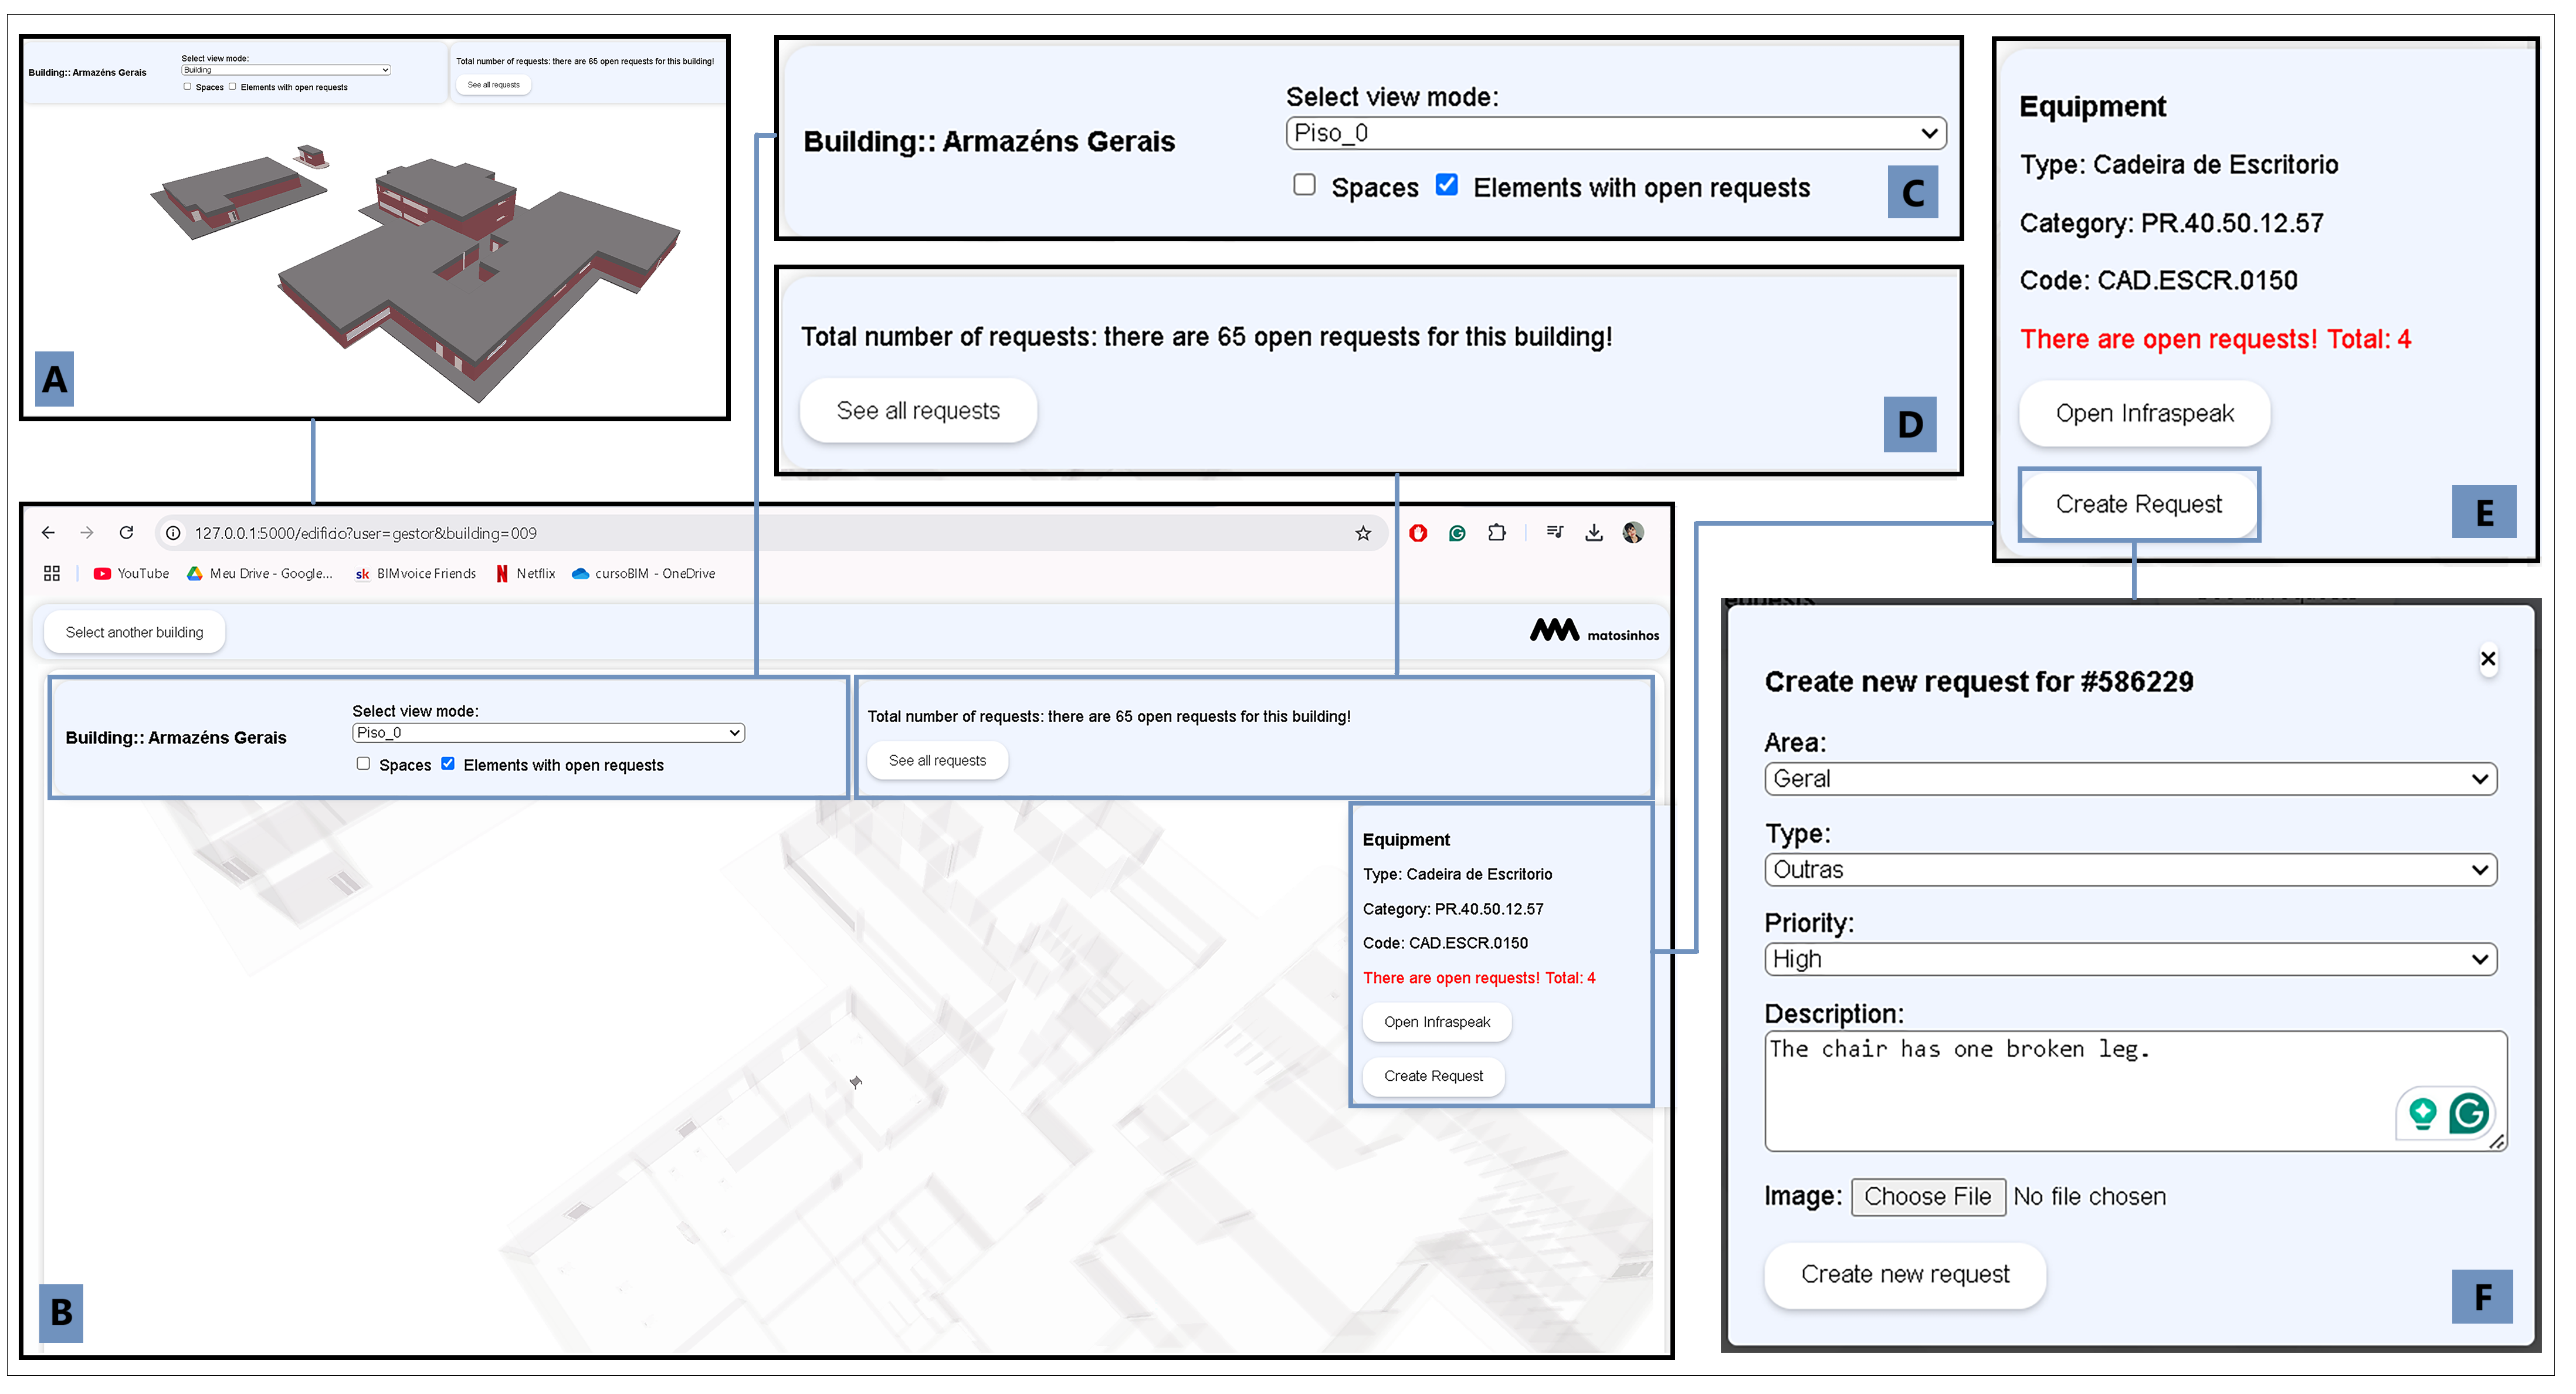
\includegraphics[width=\textwidth]{Images/plataforma.png}
    \caption{Web platform}
    \label{fig_plataforma}
\end{figure*}

\section{Discussion and conclusion}
\label{sec:conclusion}

This work supports the implementation of BIM for FM, specifically in integrating the methodology with existing management platforms. Challenges emerged during the developments regarding the unique identifiers related to CMMatosinhos' inventory, which did not uniquely identify assets, implying the necessity of combining codes for this objective. An iterative process with CMMatosinhos helped overcome these limitations, leading to optimizations that improved user experience, such as automated mapping of elements that reduced information update times. This challenge also demonstrated the necessity for the operating section to organize its inventory in a way that supports automatization. The IFCjs library allowed diverse visualization modes for the models and data extraction to allow integration with the IMMP platform. This work demonstrates a real case of applying BIM to improve building operations by integrating an information model with existing management systems, offering a framework for future integration processes.

\section{Acknowledgements}
\label{sec:acknowledgements}

This work was partly financed by FCT / MCTES through national funds (PIDDAC) under the R\&D Unit Institute for Sustainability and Innovation in Structural Engineering (ISISE), under reference UIDB / 04029/2020 (doi.org/10.54499/UIDB/04029/2020), and under the Associate Laboratory Advanced Production and Intelligent Systems ARISE under reference LA/P/0112/2020. This work is also financed by national funds through FCT – Foundation for Science and Technology, under grant agreement PRT/BD/154416/2023 attributed to the 1st author, under the MIT Portugal Programme.

\bibliography{ISARC}

\end{document}
